\documentclass[a4paper,12pt,twoside]{memoir}

% Castellano
\usepackage[spanish,es-tabla]{babel}
\selectlanguage{spanish}
\usepackage[utf8]{inputenc}
\usepackage[T1]{fontenc}
\usepackage{lmodern} % scalable font
\usepackage{microtype}
\usepackage{placeins}

\RequirePackage{booktabs}
\RequirePackage[table]{xcolor}
\RequirePackage{xtab}
\RequirePackage{multirow}

% Links
\PassOptionsToPackage{hyphens}{url}\usepackage[colorlinks]{hyperref}
\hypersetup{
	allcolors = {red}
}

% Acrónimos
\usepackage[acronym]{glossaries}
\makenoidxglossaries

\newacronym{llm}{LLM}{\textit{Large Language Models}}
\newacronym{ods}{ODS}{\textit{Objetivos de Desarrollo Sostenible}}
\newacronym{ods11}{ODS11}{\textit{Ciudades y Comunidades Sostenibles}}
\newacronym{sdg}{SDG}{\textit{Sustainable Development Goals}}
\newacronym{sc}{Smart City}{\textit{Ciudades Inteligentes}}
\newacronym{sdg11}{SDG11}{\textit{Sustainable Cities and Communities}}
\newacronym{pdi}{PDI}{\textit{Punto de Interés}}
\newacronym{tfg}{TFG}{\textit{Trabajo de Fin de Grado}}
\newacronym{so}{SO}{\textit{Sistema Operativo}}
\newacronym{gps}{GPS}{\textit{Global Positioning System}}
\newacronym{sig}{GIS}{\textit{Sistemas de Información Geográfica}}

\newcommand{\autor}{Fernando Pisot Serrano}

% Ecuaciones
\usepackage{amsmath}

% Rutas de fichero / paquete
\newcommand{\ruta}[1]{{\sffamily #1}}

% Párrafos
\nonzeroparskip

% Huérfanas y viudas
\widowpenalty100000
\clubpenalty100000

% Evitar solapes en el header
\nouppercaseheads

% Imagenes
\usepackage{graphicx}
\newcommand{\imagen}[2]{
	\begin{figure}[!h]
		\centering
		\includegraphics[width=0.9\textwidth]{#1}
		\caption{#2}\label{fig:#1}
	\end{figure}
	\FloatBarrier
}

\newcommand{\imagenflotante}[2]{
	\begin{figure}%[!h]
		\centering
		\includegraphics[width=0.9\textwidth]{#1}
		\caption{#2}\label{fig:#1}
	\end{figure}
}



% El comando \figura nos permite insertar figuras comodamente, y utilizando
% siempre el mismo formato. Los parametros son:
% 1 -> Porcentaje del ancho de página que ocupará la figura (de 0 a 1)
% 2 --> Fichero de la imagen
% 3 --> Texto a pie de imagen
% 4 --> Etiqueta (label) para referencias
% 5 --> Opciones que queramos pasarle al \includegraphics
% 6 --> Opciones de posicionamiento a pasarle a \begin{figure}
\newcommand{\figuraConPosicion}[6]{%
  \setlength{\anchoFloat}{#1\textwidth}%
  \addtolength{\anchoFloat}{-4\fboxsep}%
  \setlength{\anchoFigura}{\anchoFloat}%
  \begin{figure}[#6]
    \begin{center}%
      \Ovalbox{%
        \begin{minipage}{\anchoFloat}%
          \begin{center}%
            \includegraphics[width=\anchoFigura,#5]{#2}%
            \caption{#3}%
            \label{#4}%
          \end{center}%
        \end{minipage}
      }%
    \end{center}%
  \end{figure}%
}

%
% Comando para incluir imágenes en formato apaisado (sin marco).
\newcommand{\figuraApaisadaSinMarco}[5]{%
  \begin{figure}%
    \begin{center}%
    \includegraphics[angle=90,height=#1\textheight,#5]{#2}%
    \caption{#3}%
    \label{#4}%
    \end{center}%
  \end{figure}%
}
% Para las tablas
\newcommand{\otoprule}{\midrule [\heavyrulewidth]}
%
% Nuevo comando para tablas pequeñas (menos de una página).
\newcommand{\tablaSmall}[5]{%
 \begin{table}
  \begin{center}
   \rowcolors {2}{gray!35}{}
   \begin{tabular}{#2}
    \toprule
    #4
    \otoprule
    #5
    \bottomrule
   \end{tabular}
   \caption{#1}
   \label{tabla:#3}
  \end{center}
 \end{table}
}

%
%Para el float H de tablaSmallSinColores
\usepackage{float}

%
% Nuevo comando para tablas pequeñas (menos de una página).
\newcommand{\tablaSmallSinColores}[5]{%
 \begin{table}[H]
  \begin{center}
   \begin{tabular}{#2}
    \toprule
    #4
    \otoprule
    #5
    \bottomrule
   \end{tabular}
   \caption{#1}
   \label{tabla:#3}
  \end{center}
 \end{table}
}

\newcommand{\tablaApaisadaSmall}[5]{%
\begin{landscape}
  \begin{table}
   \begin{center}
    \rowcolors {2}{gray!35}{}
    \begin{tabular}{#2}
     \toprule
     #4
     \otoprule
     #5
     \bottomrule
    \end{tabular}
    \caption{#1}
    \label{tabla:#3}
   \end{center}
  \end{table}
\end{landscape}
}

%
% Nuevo comando para tablas grandes con cabecera y filas alternas coloreadas en gris.
\newcommand{\tabla}[6]{%
  \begin{center}
    \tablefirsthead{
      \toprule
      #5
      \otoprule
    }
    \tablehead{
      \multicolumn{#3}{l}{\small\sl continúa desde la página anterior}\\
      \toprule
      #5
      \otoprule
    }
    \tabletail{
      \hline
      \multicolumn{#3}{r}{\small\sl continúa en la página siguiente}\\
    }
    \tablelasttail{
      \hline
    }
    \bottomcaption{#1}
    \rowcolors {2}{gray!35}{}
    \begin{xtabular}{#2}
      #6
      \bottomrule
    \end{xtabular}
    \label{tabla:#4}
  \end{center}
}

%
% Nuevo comando para tablas grandes con cabecera.
\newcommand{\tablaSinColores}[6]{%
  \begin{center}
    \tablefirsthead{
      \toprule
      #5
      \otoprule
    }
    \tablehead{
      \multicolumn{#3}{l}{\small\sl continúa desde la página anterior}\\
      \toprule
      #5
      \otoprule
    }
    \tabletail{
      \hline
      \multicolumn{#3}{r}{\small\sl continúa en la página siguiente}\\
    }
    \tablelasttail{
      \hline
    }
    \bottomcaption{#1}
    \begin{xtabular}{#2}
      #6
      \bottomrule
    \end{xtabular}
    \label{tabla:#4}
  \end{center}
}

%
% Nuevo comando para tablas grandes sin cabecera.
\newcommand{\tablaSinCabecera}[5]{%
  \begin{center}
    \tablefirsthead{
      \toprule
    }
    \tablehead{
      \multicolumn{#3}{l}{\small\sl continúa desde la página anterior}\\
      \hline
    }
    \tabletail{
      \hline
      \multicolumn{#3}{r}{\small\sl continúa en la página siguiente}\\
    }
    \tablelasttail{
      \hline
    }
    \bottomcaption{#1}
  \begin{xtabular}{#2}
    #5
   \bottomrule
  \end{xtabular}
  \label{tabla:#4}
  \end{center}
}



\definecolor{cgoLight}{HTML}{EEEEEE}
\definecolor{cgoExtralight}{HTML}{FFFFFF}

%
% Nuevo comando para tablas grandes sin cabecera.
\newcommand{\tablaSinCabeceraConBandas}[5]{%
  \begin{center}
    \tablefirsthead{
      \toprule
    }
    \tablehead{
      \multicolumn{#3}{l}{\small\sl continúa desde la página anterior}\\
      \hline
    }
    \tabletail{
      \hline
      \multicolumn{#3}{r}{\small\sl continúa en la página siguiente}\\
    }
    \tablelasttail{
      \hline
    }
    \bottomcaption{#1}
    \rowcolors[]{1}{cgoExtralight}{cgoLight}

  \begin{xtabular}{#2}
    #5
   \bottomrule
  \end{xtabular}
  \label{tabla:#4}
  \end{center}
}




\graphicspath{ {./img/} }

% Capítulos
\chapterstyle{bianchi}
\newcommand{\capitulo}[2]{
	\setcounter{chapter}{#1}
	\setcounter{section}{0}
	\setcounter{figure}{0}
	\setcounter{table}{0}
	\chapter*{#2}
	\addcontentsline{toc}{chapter}{#2}
	\markboth{#2}{#2}
}

% Apéndices
\renewcommand{\appendixname}{Apéndice}
\renewcommand*\cftappendixname{\appendixname}

\newcommand{\apendice}[1]{
	%\renewcommand{\thechapter}{A}
	\chapter{#1}
}

\renewcommand*\cftappendixname{\appendixname\ }

% Formato de portada
\makeatletter
\usepackage{xcolor}
\newcommand{\tutor}[1]{\def\@tutor{#1}}
\newcommand{\course}[1]{\def\@course{#1}}
\definecolor{cpardoBox}{HTML}{E6E6FF}
\def\maketitle{
  \null
  \thispagestyle{empty}
  % Cabecera ----------------
\noindent
\includegraphics[width=\textwidth]{cabecera}\vspace{1cm}%
  \vfill
  % Título proyecto y escudo informática ----------------
  \colorbox{cpardoBox}{%
    \begin{minipage}{.8\textwidth}
      \vspace{.5cm}\Large
      \begin{center}
      \textbf{TFG del Grado en Ingeniería Informática}\vspace{.6cm}\\
      \textbf{\LARGE\@title{}}
      \end{center}
      \vspace{.2cm}
    \end{minipage}

  }%
  \hfill\begin{minipage}{.20\textwidth}
    
\includegraphics[width=\textwidth]{escudoInfor}
  \end{minipage}
  \vfill
  % Datos de alumno, curso y tutores ------------------
  \begin{center}%
  {%
    \noindent\LARGE
    Presentado por \@author{}\\ 
    en Universidad de Burgos --- \@date{}\\
    Tutor: \@tutor{}\\
  }%
  \end{center}%
  \null
  \cleardoublepage
  }
\makeatother


% Datos de portada
\title{Aplicación móvil para la generación de rutas turísticas sostenibles propuestas por modelos de lenguaje de gran escala \\Documentación Técnica}
\author{Fernando Pisot Serrano}
\tutor{Carlos López Nozal}
\date{\today}

\begin{document}

\maketitle



\cleardoublepage


%%%%%%%%%%%%%%%%%%%%%%%%%%%%%%%%%%%%%%%%%%%%%%%%%%%%%%%%%%%%%%%%%%%%%%%%%%%%%%%%%%%%%%%%



\frontmatter


\clearpage

% Indices
\tableofcontents

\clearpage

\listoffigures

\clearpage

\listoftables

\clearpage

\mainmatter

\appendix

\apendice{Plan de Proyecto Software}

\section{Introducción}
El Plan de Proyecto Software es el documento clave que dirige el proceso de desarrollo de la aplicación móvil creada. Este apéndice tiene como objetivo detallar los aspectos críticos de la planificación y gestión del proyecto, asegurando una implementación eficiente y efectiva.
La planificación temporal del proyecto se ha llevado a cabo con el \emph{uso de la metodología ágil} buscando dividir el desarollo en tareas, sprints e hitos que producen un resultado iterativos y bien estructurado, lo que conlleva a una mayor flexibilidad y a la adaptación más efectiva frente los cambios. 

A continuación, se determinará la viabilidad, que reflejará los \emph{recursos humanos y materiales}, así como los costes asociados necesarios para su valoración. La viabilidad incluirá una estimación de los fondos que se basarán en el salario de un trabajador de la imaginación, así como un análisis de los posibles riesgos y su mitigación. Los aspectos económicos y técnicos de la viabilidad son fundamentales, ya que de ellos depende de que el proyecto esté en los límites establecidos y cumpla con los objetivos propuestos.

Este plan es esencial para la gestión del proyecto ya que sirve como una guía detallada, ayudando así a identificar y mitigar riesgos así como a la utilización eficaz de los recursos. Con el enfoque estructurado y ágil, proporcionado por este plan, el equipo de desarrollo podría entregar un producto de alta calidad que, además, cumplirá con el nivel de satisfacción alcanzado entre los usuarios o clientes. 
\section{Planificación temporal}
 Como se ha mencionado anteriormente, la planificación temporal del proyecto se ha llevado a cabo con el uso de metodología ágil: se basa en la división del desarrollo en tareas, sprints e hitos que producen un resultado iterativo y bien estructurado. Esto conlleva una mayor flexibilidad y a la adaptación más efectiva frente a los cambios.

 Algunas herramientas utilizadas para la planificación temporal han sido GitHub y Zube. Ésta última ha permitido la organización de las tareas en tableros Kanban. El uso de GitHub ha permitido gestionar un control de versiones.

 A continuación veremos como la planificación temporal se ha llevado a cabo en diferentes sprints, cómo se ha ido iterando en las diferentes partes del proyecto y cómo se han ido cumpliendo los hitos propuestos. Para ello se mostrarán diferentes diagramas basadas en métricas ágiles.

 Cada tarea se ha dividido en diferentes historias de usuario, que se han ido completando en cada sprint. Cada sprint ha tenido una duración de una o dos semanas, y se han ido completando las tareas propuestas en cada uno de ellos.
 Un ejemplo se puede observar en la siguiente figura ~\ref{fig:issue12}
 \imagen{issue12}{Tarea 12 mostrada en GitHub con la descripción, hito y etiquetas de la tarea a realizar.}

Gracias al uso de la herramienta Zube, se ha podido llevar un control de las tareas a realizar, las tareas completadas y las tareas pendientes. Además, se ha podido llevar un control de los hitos propuestos y de las historias de usuario completadas en cada sprint. Un ejemplo de ello se puede observar en la siguiente figura ~\ref{fig:sprint1}
\imagen{sprint1}{Tablero Kanban de Zube con la gestión de tareas del Sprint 1.}

\subsection{\textit{Hitos}}
Los hitos o milestones son puntos de referencia que marcan el final de un conjunto de tareas. En este proyecto se han definido los siguientes hitos:

\begin{itemize}

    \item \textbf{Kick-off} Completado el 30 de julio de 2024. Puesta en marcha del proyecto. A partir de las reuniones mantenidas con el tutor, se necesita tener todas las herramientas preparadas para empezar a desarrollar tanto la aplicación como su documentación.
    
    \item \textbf{MPV - Mínimo Producto Viable} Completado el 2 de septiembre de 2024. Se define el MVP como una aplicación móvil que sobre un mapa OSM muestre la ubicación de usuario, obtenga unos \acrshort{pdi} básicos y una ruta que las una.

    \item \textbf{Checkpoint 1 de documentación} Completado el 2 de septiembre de 2024. Este milestone agrupa las tareas relacionadas con la creación y actualización de la documentación del proyecto hasta la reunión con el tutor el 1 de septiembre de 2024.

    El objetivo es tener una documentación suficiente para que el tutor pueda dar feedback acerca de la misma y poder corregir errores.

    \item \textbf{Prototipo con tours generados por LLM} Completado el 1 de octubre de 2024. El objetivo es transitar desde una aplicación inicial capaz de mostrar lugares y rutas en un mapa, hacia una aplicación que sea capaz de conseguir que estos mismos marcadores y polilíneas sean generados a través de un LLM. \label{hito:prototipo_llm}
    
    \item \textbf{Prototipo Prompting} Completado el 15 de octubre de 2024. Este prototipo se puede realizar en un cuaderno Jupyter y su objetivo es mostrar la evolución en el prompt que dará como resultado unos \acrshort{pdi} de mayor calidad.
    
    \item \textbf{Desarrollo de aplicación completo} Completado el 12 de noviembre de 2024. Se consideran todas las funcionalidades que debe tener la aplicación a presentar como completadas.
    
\end{itemize}

\subsection{Organización en \textit{Sprints}}

Al comenzar este proyecto durante periodo no lectivo se realizaron los Sprint con variación de tiempo de una o dos semanas en función de la planificación personal. Una vez comenzado el curso y con la ayuda del tutor se realizaron reuniones que han servido para, siguiendo la metodología \textit{Agile}, revisar el Sprint anterior, planificar el siguiente y hacer una pequeña retrospectiva para mejorar el trabajo conjunto.


\begin{itemize}
    \item \textbf{Sprint 0 - Kick-off(22/07/2024 - 29/07/2024):} Después de las reuniones con el tutor, se establecen los objetivos del proyecto y se comienza a trabajar en la puesta en marcha del proyecto. Se establecen las herramientas a utilizar y se comienza a trabajar en la documentación del proyecto. 33 puntos de historia en 5 tareas.
    
    ~\ref{fig:bd-kick-off sprint}
    \imagen{bd-kick-off sprint}{Figura burndown del Sprint Kick-off.}

    \item \textbf{Sprint 1 - Investigación LLM y desarrollo básico de aplicación con mapa (29/07/2024 - 05/08/2024):} Con las herramientas y una idea previa establecida, es el momento de empezar a desarrollar.
    

    Objetivos: seguir formándome en LLM y las opciones que pueda implementar en el prototipo de prompt.
    Empezar a desarrollar la aplicación móvil con las características básicas.
    Aprender a documentar sprints, indicar elementos que tendré que documentar y aquellos que tenga claro ir documentando para hacer un avance significativo que pueda evaluar mi tutor.
    ~\ref{fig:bd-s1}
    \imagen{bd-s1}{Figura burndown del Sprint 1: Investigación LLM y desarrollo básico de aplicación con mapa.}
    
    \item \textbf{Sprint 2 - Implementación solución GIS (05/08/2024 - 12/08/2024):} A partir del concepto básico, se añaden pequeñas mejoras en los tres aspectos del proyecto.
    
    Objetivos: mejorar el prototipo de prompting del cuaderno Jupyter hasta incorporar un sistema RAG, incluir marcadores al mapa en cuanto al desarrollo y continuar con la documentación.
    ~\ref{fig:bd-s2}
    \imagen{bd-s2}{Figura burndown del Sprint 2: Implementación solución GIS.}
    
    \textit{Dificultades encontradas}: la documentación me hizo perder mucho tiempo debido a problemas con las librerías, después de mucho tiempo reinicié el proyecto desde la plantilla dada, insertando el texto, lo que solucionó el problema. En cuanto al diseño de la aplicación, el desarrollo fue lento al tener que evaluar diferentes opciones ya que la mayoría de fuentes utilizan mapas de Google, opción que se quería descartar.
 

    \item \textbf{Sprint 3 - MPV(12/08/2024 - 22/08/2024):} Este sprint fue más largo que los anteriores para mejorar el resultado final ya que la intención era dejar el proyecto en un estado de revisión lo más completo posible para afrontar la reunión prevista para inicio de septiembre con el tutor del mismo. Al intentar desarrollar la tecnología de enrutado del usuario se comprendió lo que ya se intuía en el sprint anterior y es que basar el trabajo en servicios de Google iba a reportar en un desarrollo más fácil y un resultado más robusto y fiable como se justifica en la sección 5 de la memoria de este \acrshort{tfg}.
~\ref{fig:bd-s3}
\imagen{bd-s3}{Figura burndown del Sprint 3: MPV.}
    
    \item \textbf{Sprint 4 - Servicios MapBox y LLM, preparación reunión inicio curso.(22/08/2024 - 02/09/2024):} El objetivo es mostrar la versión más completa de la aplicación, la documentación y ahondar en el uso de nuevas herramientas como Figma como herramienta de diseño de aplicaciones y LangFlow a la hora de utilizar otro modelo de prototipo.
    ~\ref{fig:bd-s4}
    \imagen{bd-s4}{Figura burndown del Sprint 4: Servicios MapBox y LLM, preparación reunión inicio curso.}
    
\item \textbf{Sprint 5 - Aplicación con origen de datos LLM (Preparación y documentación) (04/09/2024 - 14/09/2024):} Después de la reunión con el tutor de inicio de septiembre y habiendo cumplido los objetivos de los primeros hitos se decide continuar intentando alcanzar el hito \ref{hito:prototipo_llm}. Para ello se prepara y documenta primero en este sprint el desarrollo necesario.
~\ref{fig:bd-s5}
\imagen{bd-s5}{Figura burndown del Sprint 5: Aplicación con origen de datos LLM (Preparación y documentación).}

\item \textbf{Sprint 6 - Desarrollo y Finalización prototipo google\_generative\_ai como LLM (18/09/2024-01/10/2024):} Habiendo encontrado una solución óptima al modelo LLM a utilizar se propone realizar un prototipo que implemente la interfaz de usuario y su conexión con el modelo LLM. En los diferentes apartados encontramos. Se trata de un sprint de prominente desarrollo de la aplicación. Se consiguió reestructurar todo el código centralizando labores de gestión del tour generado y sus \acrshort{pdi} manteniendo la modularidad del código.
~\ref{fig:bd-s6}
\imagen{bd-s6}{Figura burndown del Sprint 6:  Desarrollo y Finalización prototipo google\_generative\_ai como LLM.}
	
\item \textbf{S7 - Consolidación y Calidad (02/10/2024 - 22/10/2024)} Habiendo cumplido el hito \ref{hito:prototipo_llm} y teniendo una aplicación con muchas funcionalidades buscadas, durante este sprint se busca consolidar el código y dotarlo de una calidad y mantenimiento con herramientas de soporte como Sonar Cloud o Logger.
~\ref{fig:bd-s7}
\imagen{bd-s7}{Figura burndown del Sprint 7: Consolidación y Calidad.}

\item \textbf{S8 - Cobertura de tests y guardado de rutas (23/10/2024 - 12/11/2024):} Se procede a implementar las últimas funcionalidades del desarrollo de la aplicación. Además, se busca que la integración con sonarcloud confirme que se trabaja con un standard de calidad para lo que se necesita la cobertura de tests y por último se retoma el trabajo de documentación. 

\end{itemize}

\subsection{Métricas Ágiles}
Gracias al uso de Zube se emplean fácilmente diferentes métricas ágiles que han sido vitales para la evaluación del desarrollo de la aplicación y su organización a través de los sprints citados. Algunos de los artefactos usados son los siguientes:
\subsubsection{Gráficos burnup / burndown} 
Muestran a lo largo del tiempo de un sprint la evolución de tareas realizadas por el equipo de desarrollo. En la explicación de los sprints se pueden ver los gráficos asociados al mismo
\imagen{burnup-s6}{Gráfico Burnup del Sprint 6}{1}
\subsubsection{Gráfico de velocidad} 
Permite comprobar el trabajo realizado en los diferentes sprints de manera que resulte lo más constante posible.


\section{Estudio de viabilidad}

\subsection{Viabilidad económica}

\subsection{Viabilidad legal}



\apendice{Especificación de Requisitos}

\section{Introducción}
En esta sección se presentan los requisitos de la aplicación, abordando tanto los objetivos generales como los específicos del proyecto. Se incluye un catálogo detallado de los requisitos funcionales y no funcionales, que definen el comportamiento y las características técnicas de la aplicación. Además, se proporciona una especificación detallada de los requisitos a través de tablas de casos de uso, complementadas con su respectivo diagrama de casos de uso, lo que facilita una comprensión clara de las interacciones principales de los usuarios con el sistema.


\section{Objetivos generales}
La misión fundamental de este proyecto persigue conseguir los siguientes propósitos:
\begin{itemize}
	\item \textbf{Fomentar el turismo sostenible:} Facilitar a los usuarios la exploración de ciudades promoviendo al mostrar rutas no motorizadas y modos de transporte como caminar y el uso de bicicletas.
	
	\item \textbf{Optimización de experiencias turísticas personalizadas:} Ofrecer a los usuarios rutas personalizadas que se ajusten a sus intereses y preferencias, proporcionando información detallada y relevante sobre los puntos de interés seleccionados.
	
	\item \textbf{Promover el uso de tecnologías inteligentes en el turismo:} Utilizar tecnologías avanzadas como servicios GIS, Google Places y LLMs para mejorar la experiencia del usuario, facilitando la generación automática de rutas y la obtención de información actualizada sobre los destinos turísticos.
	
	\item \textbf{Mejorar la accesibilidad a la información turística:} Proporcionar una plataforma fácil de usar que permita a los usuarios acceder rápidamente a descripciones, fotos y otros datos sobre los puntos de interés, mejorando su experiencia de exploración en las ciudades.
	
	\item \textbf{Rutas generadas sin intereses comerciales:} Generar rutas turísticas sin influencias comerciales, ofreciendo una experiencia imparcial y auténtica, en contraste con otras aplicaciones de recomendaciones de viajes.
\end{itemize}

\section{Catálogo de requisitos}
\subsection{Requisitos funcionales}
\begin{itemize}
	\item \textbf{RF-1 Solicitar permisos de uso de GPS:} La aplicación solicitará el permiso para acceder al GPS cuando se inicie por primera vez, ya que es necesario para calcular y mostrar la ubicación del usuario en tiempo real.
	
	\item \textbf{RF-2 Solicitud de activación de GPS:} Si el GPS está desactivado, la aplicación redirigirá a una pantalla que indicará al usuario la necesidad de activarlo para el correcto funcionamiento de la aplicación.
	
	\item \textbf{RF-3 Activación/Desactivación de seguimiento de usuario:} La aplicación mostrará en tiempo real el recorrido del usuario en el mapa, y este seguimiento podrá activarse o desactivarse en cualquier momento mediante un botón.
	
	\item \textbf{RF-4 Centrar la situación actual del usuario sobre el mapa:} El usuario podrá centrar manualmente su posición en el mapa mediante un botón dedicado. Además, existe la opción de fijar la ubicación del usuario en el centro del mapa durante su recorrido.
	
	\item \textbf{RF-5 Selección de Tour:} El usuario rellenará un formulario indicando el lugar que desea visitar, la cantidad de puntos de interés que quiere ver, sus preferencias de transporte (a pie o bicicleta), sus intereses, y el tiempo máximo que quiere dedicar a la ruta.
	
	\item \textbf{RF-6 Cálculo de información a través de un LLM:} La aplicación usará un servicio Gemini para generar los puntos de interés de acuerdo con las preferencias del usuario. Además, un servicio Google Places mejorará los datos proporcionando descripciones, fotos, URLs, ratings y número de votos de los POI.
	
	\item \textbf{RF-7 Eliminación de POI:} El usuario podrá eliminar puntos de interés tanto desde la pantalla del mapa como desde el resumen de la ruta. Cada vez que un POI es eliminado o añadido, la ruta se recalcula automáticamente para ofrecer el trayecto más óptimo.
	
	\item \textbf{RF-8 Cálculo de ruta optimizada:} La aplicación calculará la ruta más corta que conecte los puntos de interés seleccionados por el usuario, adaptándose al medio de transporte elegido (a pie o bicicleta).
	
	\item \textbf{RF-9 Capacidad de añadir un POI:} El usuario podrá agregar manualmente un lugar introduciendo su nombre en la barra de búsqueda. Si el lugar existe en los servicios de Google, será añadido automáticamente a la ruta; de lo contrario, no se tomará ninguna acción.
	
	\item \textbf{RF-10 Unirse a Eco City Tour:} El usuario podrá unirse a la ruta existente en cualquier momento. La aplicación calculará la ruta más corta para conectarlo con el tour.
	
	\item \textbf{RF-11 Mejora de los puntos de interés con servicio de obtención de información:} Los datos de los puntos de interés se enriquecerán con información adicional obtenida de Google Places, incluyendo ratings, imágenes, URL y número de votos, mejorando la experiencia del usuario.
	
	\item \textbf{RF-12 Guardado y carga de las rutas turísticas:} el usuario podrá guardar los tours que quiera y tendrá acceso a los mismos desde la pantalla de configuración del Eco City Tour.
	
\end{itemize}

\subsection{Requisitos no funcionales}
\begin{itemize}
	\item \textbf{RNF-1 Rendimiento:} la aplicación debe demostrar un tiempo de respuesta aceptable para que su manejo sea fluido y la carga de datos sea razonable al enlazar varios servicios asíncronos, de tal manera que no se perjudique la experiencia de usuario. 
	\item \textbf{RNF-2 Usabilidad:} Eco City Tours debe ser intuitiva y fácil de entender y utilizar.
	\item \textbf{RNF-3 Disponibilidad:} la aplicación debe estar disponible independientemente de la localización del usuario.
	\item \textbf{RNF-4 Mantenibilidad:} la aplicación debe ser fácilmente modificable debido a su carácter modular, facilitando el mantenimiento para el desarrollador. Además, \textbf{el uso de SonarCloud} ayuda a asegurar la calidad del código mediante el análisis continuo, lo que permite identificar y corregir errores potenciales y optimizar el código, favoreciendo así la mantenibilidad a largo plazo.
	
	\item \textbf{RNF-5 Escalabilidad:} Eco City Tours debe ser capaz de gestionar eficientemente un crecimiento continuo en el número de usuarios, adaptándose sin problemas para ofrecer un rendimiento óptimo incluso en situaciones de alta demanda.
	\item \textbf{RNF-6 Soporte:} la aplicación debe funcionar en versiones actuales de Android sin problemas de rendimiento o fallos en alguna de sus funcionalidades
\end{itemize}
\clearpage

\section{Especificación de requisitos}
\begin{figure}[H]
	\centering
	\includegraphics[scale=0.6]{CU00-Gestión-de-GPS}
	\caption{Diagrama de caso de uso CU00 - Configuración GPS}
	\label{fig:CU00-Gestión-de-GPS}
\end{figure}



Este caso de uso es fundamental, ya que sin el permiso de GPS o la activación del sensor, el resto de funcionalidades de la aplicación no pueden ejecutarse. Para mayor claridad y facilitar la lectura de los diagramas restantes, se presenta por separado, destacando su papel como requisito previo para las demás operaciones.

\begin{table}[p]
	\centering
	\begin{tabularx}{\linewidth}{ p{0.21\columnwidth} p{0.71\columnwidth} }
		\toprule
		\textbf{CU00}    & \textbf{Configuración GPS} \\
		\toprule
		\textbf{Versión}              & 1.0    \\
		\textbf{Actor}                & Usuario, Sistema \\
		\textbf{Autor}                & \autor \\
		\textbf{Descripción}          & Configura la aplicación para tener acceso a la ubicación mediante GPS. \\
		\textbf{Precondición}         & La aplicación está instalada y abierta por primera vez o tras haber revocado permisos anteriormente. \\
		\textbf{Acciones}             &
		\begin{enumerate}
			\def\labelenumi{\arabic{enumi}.}
			\tightlist
			\item La aplicación solicita permiso para el uso del GPS.
			\item El usuario concede el permiso.
			\item La aplicación detecta si el GPS está activado.
			\item Si el GPS no está activado, solicita al usuario activarlo.
		\end{enumerate}\\
		\textbf{Postcondición}        & La aplicación tiene acceso a la ubicación en tiempo real. \\
		\textbf{Excepciones}          & 
		\begin{itemize}
			\tightlist
			\item El usuario no concede el permiso de GPS.
			\item El usuario no activa el GPS cuando se le solicita.
		\end{itemize}\\
		\textbf{Importancia}          & Alta \\
		\bottomrule
	\end{tabularx}
	\caption{CU00 Configuración GPS}
\end{table}

\FloatBarrier



\begin{figure}[H]
	\centering
	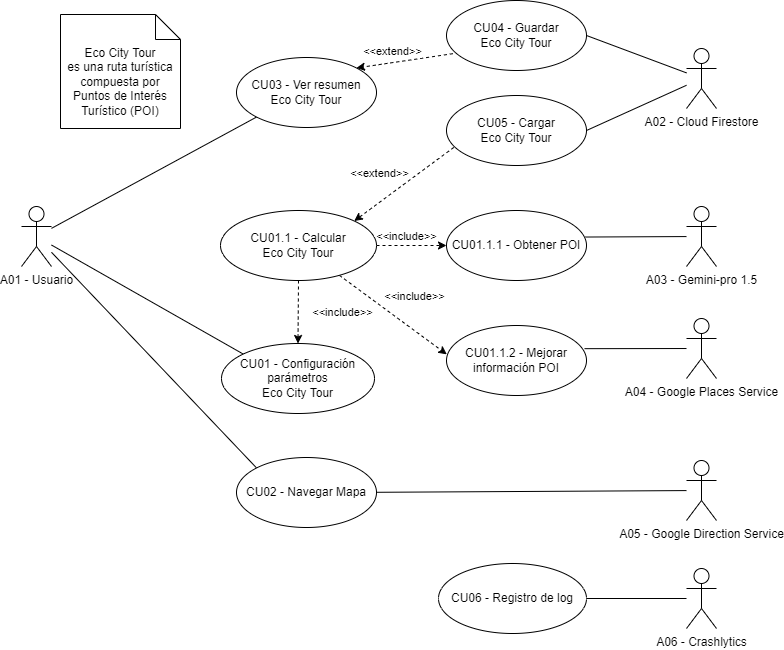
\includegraphics[scale=0.6]{casos-de-uso}
	\caption{Diagrama de casos de uso general de Eco City Tours}
	\label{fig:casos-de-uso}
\end{figure}




\begin{table}[p]
	\centering
	\begin{tabularx}{\linewidth}{ p{0.21\columnwidth} p{0.71\columnwidth} }
		\toprule
		\textbf{CU01}    & \textbf{Configuración parámetros Eco City Tour} \\
		\toprule
		\textbf{Versión}              & 1.0    \\
		\textbf{Actor}                & A01 \\
		\textbf{Autor}                & \autor \\
		\textbf{Descripción}          & Configurar los parámetros necesarios para generar un Eco City Tour personalizado según las preferencias del usuario. \\
		\textbf{Precondición}         & El usuario accede a la pantalla de configuración. \\
		\textbf{Acciones}             &
		\begin{enumerate}
			\def\labelenumi{\arabic{enumi}.}
			\tightlist
			\item El usuario completa el formulario de preferencias, incluyendo el lugar, número de POIs, medio de transporte y tiempo máximo.
		\end{enumerate}\\
		\textbf{Postcondición}        & Los parámetros quedan configurados y listos para generar la ruta. \\
		\textbf{Excepciones}          & 
		\begin{itemize}
			\tightlist
			\item El usuario no completa el formulario de configuración.
			\item Error en la carga de los datos de configuración.
		\end{itemize}\\
		\textbf{Importancia}          & Alta \\
		\bottomrule
	\end{tabularx}
	\caption{CU01 Configuración parámetros Eco City Tour}
\end{table}

\begin{table}[p]
	\centering
	\begin{tabularx}{\linewidth}{ p{0.21\columnwidth} p{0.71\columnwidth} }
		\toprule
		\textbf{CU01.1}    & \textbf{Calcular Eco City Tour} \\
		\toprule
		\textbf{Versión}              & 1.0    \\
		\textbf{Actor}                & A03, A04, A05 \\
		\textbf{Autor}                & \autor \\
		\textbf{Descripción}          & Generar una ruta optimizada conectando los puntos de interés seleccionados en función de las preferencias del usuario. \\
		\textbf{Precondición}         & Los parámetros han sido configurados correctamente. \\
		\textbf{Acciones}             &
		\begin{enumerate}
			\def\labelenumi{\arabic{enumi}.}
			\tightlist
			\item El usuario confirma la configuración de preferencias.
			\item El sistema consulta un LLM para obtener \acrshort{pdi} basados en las preferencias del usuario.
			\item El sistema envía los \acrshort{pdi} a Google Places para obtener información mejorada.
			\item El sistema consulta un servicio de optimización de rutas para generar la ruta optimizada.
		\end{enumerate}\\
		\textbf{Postcondición}        & La ruta optimizada es calculada y lista para ser visualizada. \\
		\textbf{Excepciones}          & 
		\begin{itemize}
			\tightlist
			\item Fallo en la conexión con el LLM.
			\item Error en el servicio de optimización de rutas.
		\end{itemize}\\
		\textbf{Importancia}          & Alta \\
		\bottomrule
	\end{tabularx}
	\caption{CU01.1 Calcular Eco City Tour}
\end{table}

\begin{table}[p]
	\centering
	\begin{tabularx}{\linewidth}{ p{0.21\columnwidth} p{0.71\columnwidth} }
		\toprule
		\textbf{CU02}    & \textbf{Navegar Mapa} \\
		\toprule
		\textbf{Versión}              & 1.0    \\
		\textbf{Autor}                & \autor \\
		\textbf{Actor}                & A01 \\
		\textbf{Descripción}          & El usuario puede desplazarse y explorar el mapa interactivo de la aplicación. \\
		\textbf{Precondición}         & El mapa está visible. \\
		\textbf{Acciones}             &
		\begin{enumerate}
			\def\labelenumi{\arabic{enumi}.}
			\tightlist
			\item El usuario explora el mapa desplazándose y haciendo zoom.
		\end{enumerate}\\
		\textbf{Postcondición}        & El usuario navega por el mapa para observar los POI y la ruta. \\
		\textbf{Importancia}          & Media \\
		\bottomrule
	\end{tabularx}
	\caption{CU02 Navegar Mapa}
\end{table}

\begin{table}[p]
	\centering
	\begin{tabularx}{\linewidth}{ p{0.21\columnwidth} p{0.71\columnwidth} }
		\toprule
		\textbf{CU03}    & \textbf{Ver resumen Eco City Tour} \\
		\toprule
		\textbf{Versión}              & 1.0    \\
		\textbf{Actor}                & A01 \\
		\textbf{Autor}                & \autor \\
		\textbf{Descripción}          & Muestra un resumen de la ruta generada, incluyendo la distancia, duración y medio de transporte. \\
		\textbf{Precondición}         & La ruta ha sido generada. \\
		\textbf{Acciones}             &
		\begin{enumerate}
			\def\labelenumi{\arabic{enumi}.}
			\tightlist
			\item El usuario accede a la pantalla de resumen.
			\item La aplicación muestra los detalles de la ruta, incluyendo distancia total, tiempo estimado y transporte elegido.
		\end{enumerate}\\
		\textbf{Postcondición}        & El resumen es visible para el usuario. \\
		\textbf{Excepciones}          & 
		\begin{itemize}
			\tightlist
			\item Error en la carga de los datos de la ruta.
		\end{itemize}\\
		\textbf{Importancia}          & Baja \\
		\bottomrule
	\end{tabularx}
	\caption{CU03 Ver resumen Eco City Tour}
\end{table}

\begin{table}[p]
	\centering
	\begin{tabularx}{\linewidth}{ p{0.21\columnwidth} p{0.71\columnwidth} }
		\toprule
		\textbf{CU04}    & \textbf{Guardar Eco City Tour} \\
		\toprule
		\textbf{Versión}              & 1.0    \\
		\textbf{Actor}                & A01, A02 \\
		\textbf{Autor}                & \autor \\
		\textbf{Descripción}          & Permite al usuario guardar la ruta generada para acceder a ella en el futuro. \\
		\textbf{Precondición}         & La ruta ha sido generada. \\
		\textbf{Acciones}             &
		\begin{enumerate}
			\def\labelenumi{\arabic{enumi}.}
			\tightlist
			\item El usuario selecciona la opción de guardar la ruta.
		\end{enumerate}\\
		\textbf{Postcondición}        & La ruta queda guardada en el sistema. \\
		\textbf{Excepciones}          & 
		\begin{itemize}
			\tightlist
			\item Error en el guardado de la ruta.
			\item Problemas de conexión con la base de datos.
		\end{itemize}\\
		\textbf{Importancia}          & Media \\
		\bottomrule
	\end{tabularx}
	\caption{CU04 Guardar Eco City Tour}
\end{table}

\begin{table}[p]
	\centering
	\begin{tabularx}{\linewidth}{ p{0.21\columnwidth} p{0.71\columnwidth} }
		\toprule
		\textbf{CU05}    & \textbf{Cargar Eco City Tour} \\
		\toprule
		\textbf{Versión}              & 1.0    \\
		\textbf{Actor}                & A01, A02 \\
		\textbf{Autor}                & \autor \\
		\textbf{Descripción}          & Permite al usuario cargar una ruta guardada previamente. \\
		\textbf{Precondición}         & El usuario ha guardado al menos una ruta. \\
		\textbf{Acciones}             &
		\begin{enumerate}
			\def\labelenumi{\arabic{enumi}.}
			\tightlist
			\item El usuario selecciona la opción de cargar una ruta guardada.
			\item El usuario selecciona un Eco City Tour guardado previamente que será cargado.
		\end{enumerate}\\
		\textbf{Postcondición}        & La ruta es cargada y visible en el mapa. \\
		\textbf{Excepciones}          & 
		\begin{itemize}
			\tightlist
			\item Error en la carga de la ruta guardada.
			\item Problemas de conexión con la base de datos.
		\end{itemize}\\
		\textbf{Importancia}          & Media \\
		\bottomrule
	\end{tabularx}
	\caption{CU05 Cargar Eco City Tour}
\end{table}

\begin{table}[p]
	\centering
	\begin{tabularx}{\linewidth}{ p{0.21\columnwidth} p{0.71\columnwidth} }
		\toprule
		\textbf{CU06}    & \textbf{Registro de log} \\
		\toprule
		\textbf{Versión}              & 1.0    \\
		\textbf{Actor}                & A06 \\
		\textbf{Autor}                & \autor \\
		\textbf{Descripción}          & Registra los eventos y actividades del usuario en la aplicación para fines de monitorización y depuración. \\
		\textbf{Precondición}         & La aplicación está en funcionamiento. \\
		\textbf{Acciones}             &
		\begin{enumerate}
			\def\labelenumi{\arabic{enumi}.}
			\tightlist
			\item La aplicación registra automáticamente los eventos relevantes.
		\end{enumerate}\\
		\textbf{Postcondición}        & Los eventos quedan registrados en el sistema. \\
		\textbf{Excepciones}          & 
		\begin{itemize}
			\tightlist
			\item Error en la conexión con el sistema de registros.
			\item Fallo en la escritura de los eventos en el log.
		\end{itemize}\\
		\textbf{Importancia}          & Baja \\
		\bottomrule
	\end{tabularx}
	\caption{CU06 Registro de log}
\end{table}


\FloatBarrier


\begin{figure}[H]
	\centering
	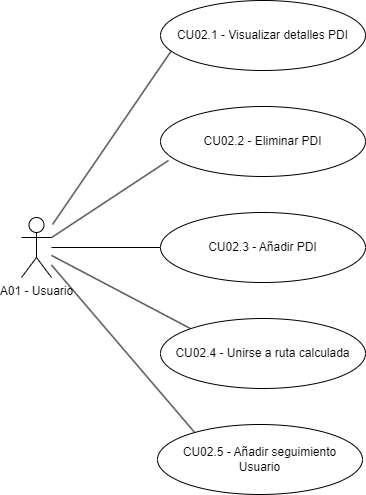
\includegraphics[scale=0.6]{CU02-Navegar-mapa}
	\caption{Diagrama de caso de uso CU02 - Navegar Mapa}
	\label{CU02-Navegar-mapa}
\end{figure}



\begin{table}[p]
	\centering
	\begin{tabularx}{\linewidth}{ p{0.21\columnwidth} p{0.71\columnwidth} }
		\toprule
		\textbf{CU02.1}    & \textbf{Visualizar detalles de puntos de interés (PDI)} \\
		\toprule
		\textbf{Versión}              & 1.0    \\
		\textbf{Actor}                & A01 \\
		\textbf{Autor}                & \autor \\
		\textbf{Descripción}          & El usuario puede obtener información detallada sobre un punto de interés seleccionado en el mapa. \\
		\textbf{Precondición}         & La ruta y los puntos de interés están visibles en el mapa. \\
		\textbf{Acciones}             &
		\begin{enumerate}
			\def\labelenumi{\arabic{enumi}.}
			\tightlist
			\item El usuario selecciona un marcador de punto de interés en el mapa.
			\item El sistema muestra la información detallada del punto de interés.
		\end{enumerate}\\
		\textbf{Postcondición}        & La información detallada del punto de interés es visible para el usuario. \\
		\textbf{Excepciones}          & 
		\begin{itemize}
			\tightlist
			\item Fallo en la carga de información del PDI debido a problemas de conectividad.
			\item Error en el servicio externo de obtención de información.
		\end{itemize}\\
		\textbf{Importancia}          & Alta \\
		\bottomrule
	\end{tabularx}
	\caption{CU02.1 Visualizar detalles de puntos de interés (PDI)}
\end{table}

\begin{table}[p]
	\centering
	\begin{tabularx}{\linewidth}{ p{0.21\columnwidth} p{0.71\columnwidth} }
		\toprule
		\textbf{CU02.2}    & \textbf{Eliminar puntos de interés (PDI)} \\
		\toprule
		\textbf{Versión}              & 1.0    \\
		\textbf{Actor}                & A01, A05 \\
		\textbf{Autor}                & \autor \\
		\textbf{Descripción}          & El usuario puede eliminar puntos de interés de la ruta desde el mapa. \\
		\textbf{Precondición}         & La ruta ha sido generada y los puntos de interés están visibles en el mapa. \\
		\textbf{Acciones}             &
		\begin{enumerate}
			\def\labelenumi{\arabic{enumi}.}
			\tightlist
			\item El usuario selecciona un punto de interés en el mapa.
			\item El sistema elimina el punto de interés de la ruta.
			\item El sistema recalcula la ruta optimizada sin el punto eliminado.
		\end{enumerate}\\
		\textbf{Postcondición}        & La ruta es recalculada sin el punto de interés eliminado. \\
		\textbf{Excepciones}          & 
		\begin{itemize}
			\tightlist
			\item Error en el recálculo de la ruta.
			\item Problemas de conectividad al intentar actualizar la ruta.
		\end{itemize}\\
		\textbf{Importancia}          & Media \\
		\bottomrule
	\end{tabularx}
	\caption{CU02.2 Eliminar puntos de interés (PDI)}
\end{table}

\begin{table}[p]
	\centering
	\begin{tabularx}{\linewidth}{ p{0.21\columnwidth} p{0.71\columnwidth} }
		\toprule
		\textbf{CU02.3}    & \textbf{Añadir puntos de interés (PDI)} \\
		\toprule
		\textbf{Versión}              & 1.0    \\
		\textbf{Actor}                & A01 \\
		\textbf{Autor}                & \autor \\
		\textbf{Descripción}          & El usuario puede añadir manualmente un nuevo \acrshort{pdi} a la ruta introduciendo su nombre en la barra de búsqueda. \\
		\textbf{Precondición}         & La ruta ha sido generada previamente. \\
		\textbf{Acciones}             &
		\begin{enumerate}
			\def\labelenumi{\arabic{enumi}.}
			\tightlist
			\item El usuario introduce el nombre de un lugar en la barra de búsqueda.
			\item El sistema muestra el resultado de la búsqueda y el usuario lo selecciona para añadirlo.
			\item El sistema recalcula la ruta optimizada incluyendo el nuevo \acrlong{pdi}.
		\end{enumerate}\\
		\textbf{Postcondición}        & El nuevo lugar es añadido a la ruta, y la ruta optimizada es recalculada. \\
		\textbf{Excepciones}          & 
		\begin{itemize}
			\tightlist
			\item El lugar no se encuentra en el servicio de búsqueda.
			\item Fallo en el recalculo de la ruta.
		\end{itemize}\\
		\textbf{Importancia}          & Baja \\
		\bottomrule
	\end{tabularx}
	\caption{CU02.3 Añadir puntos de interés (PDI)}
\end{table}

\begin{table}[p]
	\centering
	\begin{tabularx}{\linewidth}{ p{0.21\columnwidth} p{0.71\columnwidth} }
		\toprule
		\textbf{CU02.4}    & \textbf{Unirse a la ruta calculada} \\
		\toprule
		\textbf{Versión}              & 1.0    \\
		\textbf{Actor}                & A01 \\
		\textbf{Autor}                & \autor \\
		\textbf{Descripción}          & Permite al usuario unirse a una ruta previamente generada desde su ubicación actual. \\
		\textbf{Precondición}         & Una ruta ya ha sido generada y está activa. \\
		\textbf{Acciones}             &
		\begin{enumerate}
			\def\labelenumi{\arabic{enumi}.}
			\tightlist
			\item El usuario selecciona la opción para unirse a la ruta desde su ubicación actual.
			\item El sistema calcula la ruta más corta para conectar la ubicación actual del usuario con la ruta generada.
		\end{enumerate}\\
		\textbf{Postcondición}        & El usuario es guiado desde su ubicación actual hasta la ruta generada. \\
		\textbf{Excepciones}          & 
		\begin{itemize}
			\tightlist
			\item Error en el cálculo de la ruta de conexión.
			\item Problemas de conexión con el servicio de optimización de rutas.
		\end{itemize}\\
		\textbf{Importancia}          & Media \\
		\bottomrule
	\end{tabularx}
	\caption{CU02.4 Unirse a la ruta calculada}
\end{table}

\begin{table}[p]
	\centering
	\begin{tabularx}{\linewidth}{ p{0.21\columnwidth} p{0.71\columnwidth} }
		\toprule
		\textbf{CU02.5}    & \textbf{Añadir seguimiento del usuario} \\
		\toprule
		\textbf{Versión}              & 1.0    \\
		\textbf{Actor}                & A01 \\
		\textbf{Autor}                & \autor \\
		\textbf{Descripción}          & Permite al usuario activar o desactivar el seguimiento de su posición en tiempo real en el mapa. \\
		\textbf{Precondición}         & La aplicación tiene acceso a la ubicación del usuario. \\
		\textbf{Acciones}             &
		\begin{enumerate}
			\def\labelenumi{\arabic{enumi}.}
			\tightlist
			\item El usuario selecciona la opción de activar o desactivar el seguimiento de su ubicación en el mapa.
			\item El sistema ajusta el mapa para mostrar o dejar de mostrar el movimiento del usuario en tiempo real.
		\end{enumerate}\\
		\textbf{Postcondición}        & El mapa sigue o deja de seguir la posición del usuario en tiempo real. \\
		\textbf{Excepciones}          & 
		\begin{itemize}
			\tightlist
			\item Problemas de conexión con el GPS.
			\item Pérdida de señal GPS.
		\end{itemize}\\
		\textbf{Importancia}          & Baja \\
		\bottomrule
	\end{tabularx}
	\caption{CU02.5 Añadir seguimiento del usuario}
\end{table}


\apendice{Especificación de diseño}

\section{Introducción}
En este anexo, se detallan las especificaciones de diseño del proyecto, enfocadas en los aspectos fundamentales para el desarrollo de la aplicación. Se describen cómo se organizan los datos que lo componen, el diseño arquitectónico, y los procedimientos empleados. Estas especificaciones son clave para asegurar el correcto funcionamiento y la estructuración adecuada de cada uno de los elementos que componen Eco City Tours.
\section{Diseño de datos}
\imagen{clases}{Diagrama de clases de la aplicación}

\section{Diseño procedimental}

\section{Diseño arquitectónico}
\imagen{components-diagram}{Diagrama de componentes de la aplicación}
\imagen{components-simple}{Diagrama de componentes a nivel de paquetes de la aplicación}
\imagen{secuence}{Diagrama de secuencia - Generación de Eco City Tour}



\apendice{Documentación técnica de programación}

\section{Introducción}

\section{Estructura de directorios}
Se ha intentado seguir las buenas prácticas de programación adquiridas en mi formación a la hora de organizar los directorios de la siguiente manera:
\begin{itemize}
	
	\item \textbf{/}: fichero de la licencia, .gitignore y el documento \textit{Readme} con información del proyecto.
	
	\item \textbf{/project-docs/}: documentación del proyecto usando la plantilla \LaTeX  proporcionada.
	
	\item \textbf{/project-prototype/}: dos prototipos de uso de modelos LLM con ejemplos de prompting y técnicas RAG, tanto en un cuaderno Python como en LangFlow.
	
	\item \textbf{/project-app/}: se trata del proyecto Flutter creado a raiz del asistente de Visual Studio y que fue construido de manera incremental desde una aplicación vacía.
	
	
\end{itemize}

\section{Manual del programador}

\section{Compilación, instalación y ejecución del proyecto}

\section{Pruebas del sistema}

\apendice{Documentación de usuario}

\section{Introducción}

\section{Requisitos de usuarios}

\section{Instalación}

\section{Manual del usuario}



\apendice{Anexo de sostenibilización curricular}

\section{F.1. Introducción}
Durante el desarrollo del Trabajo Final de Carrera, he utilizado e implementado las disciplinas de la sostenibilidad en el diseño de una aplicación móvil. Ha sido de hecho un gran reto el tratar de generar rutas turísticas de tal manera que promocionen la sostenibilidad. Al final la solución presentada cumple con el \acrfull{ods11} fomentando principalmente la sostenibilidad de ciudades y los asentamientos humanos.

El valor principal de este \acrfull{ods}, como ya se ha tratado, radica en su papel de facilitador en la medida que, al resolver de manera integral y transversal todas las cuestiones relacionadas con la sostenibilidad de las ciudades, tiene un efecto secundario positivo en los demás \acrshort{ods}.

\section{Competencias de Sostenibilidad Adquiridas}
A lo largo del trabajo de este proyecto, he seleccionado y elaborado las competencias de sostenibilidad en las siguientes áreas:
	
	\subsection{Contextualización Crítica del Conocimiento}
	Puedo contextualizar el conocimiento adquirido y relacionarlo críticamente con los desafíos globales y locales en las áreas sociales, económicas y ambientales tan influenciadas por el turismo sostenible.
		
	\subsection{Uso Sostenible de Recursos}
	El desarrollo de la aplicación se enfocó en la utilización sostenible de los recursos. Traté de aplicar la eficiencia en el desarrollo de software al usar tecnologías que consumen la menor energía posible y al priorizar el uso de herramientas open-source, siempre que me fue posible.
		
	\subsection{Participación en Procesos Comunitarios}
	El desarrollo de esta aplicación exige una comprensión en profundidad de los procesos comunitarios. Se ha llevado a cabo por ejemplo al decir que no solo los turistas se benefician de su uso, sino que las rutas turísticas también promueven la movilidad sostenible y mejoran el bienestar de la comunidad local.
			
	\subsection{Principios Éticos y Valores de Sostenibilidad}
	 He incorporado prácticas éticas y valores de sostenibilidad en todo el trabajo descartando por ejemplo aquellas modificaciones que pudieran dar como resultado un conflicto entre la comunidad local y la turística.
				
\section{Aplicación de Competencias en el Proyecto}
				
Se utilizaron las siguientes competencias aprendidas en el desarrollo del proyecto:
	\subsection{Diseño y Funcionalidad de la Aplicación}
						
	El diseño de la aplicación ha seguido un enfoque centrado en el usuario cuyo propósito era diseñar una solución intuitiva, fácil de usar que promueva la movilidad sostenible: con ciclistas o peatones que disfruten de un viaje personalizado, uniendo los \acrfull{pdi} de una manera eficiente usando planificadores de rutas optimizados a tal efecto.
						
	\subsection{Impacto Social y Ambiental}
	La realización del proyecto busca no solo ser ventajosa para los turistas, sino que también reduce las emisiones de carbono al tiempo que permite a los miembros de la comunidad contribuir a la sostenibilidad de dicha ciudad en su conjunto.
							
	\subsection{Educación y Conciencia ambiental}
	El proyecto informará a los ciudadanos no solo con datos de rutas turísticas específicas, sino también buscará sensibilizar acerca de la movilidad sostenible y los beneficios ambientales que provienen de los dilemas referentes al transporte en los que participan.
								
\section {Conclusión}
Este Trabajo ha sido una experiencia informativa y esclarecedora para mí, tal y como indica en el artículo \cite{markiegi}, trabajar en el desarrollo de una aplicación que pone en práctica soluciones que favorecen los ODS te hace más consciente de los múltiples factores que impiden su cumplimiento. Este tiempo me ha dotado del enfoque que se necesita para enfrentar, de manera consciente y sostenible, los desafíos actuales y futuros con una visión global que trabaje activamente hacia un desarrollo sostenible y me siento capaz de liderar nuevas soluciones tecnológicas que potencien los ODS.




\bibliographystyle{plain}
\bibliography{bibliografiaAnexos}

\end{document}
